\chapter{Sistema de medición 3D}\label{chapter:proposal}

El flujo de trabajo del sistema desarrollado consta de 5 etapas: la captura de las imágenes RGB-D, seguimiento de la zona de la úlcera seleccionada de forma asistida, la segmentación, la reconstrucción 3D y las mediciones.

\section{Captura}

Uno de los objetivos fundamentales es la elaboración de un sistema de bajo costo. En el mercado existen diversas cámaras RGB-D con distintas resoluciones y características. La cámara utilizada en este trabajo es la Intel\textregistered~RealSense\texttrademark~D435i, pues es una cámara de costo justo para su precisión y calidad.

\begin{figure}[ht]
	\centering
	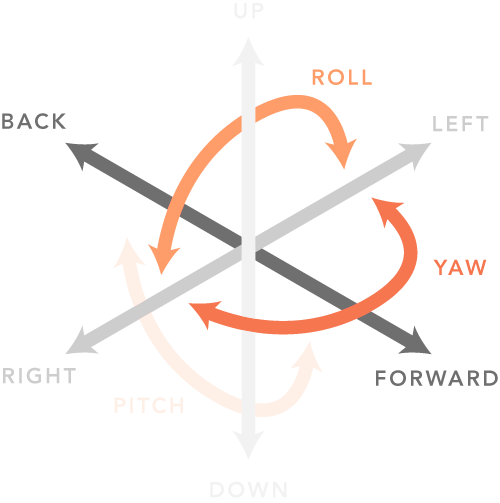
\includegraphics[width=4cm]{./Graphics/6dof.png}
	\caption{Los 6 grados de libertad en la IMU de la Intel\textregistered~RealSense\texttrademark~D435i.}
	\label{fig:6dof}
\end{figure}

El dispositivo al ser una cámara de profundidad estéreo, cuenta con dos cámaras RGB de resolución 1920 $\times$ 1080 píxeles, con un \textit{baseline} de $5,5$ cm y un sensor de láser infrarrojo que mejora la habilidad del sistema estéreo de medir profundidad. Además, cuenta de una unidad inercial (IMU, por sus siglas en inglés) que permite cuantificar el movimiento del dispositivo. El módulo IMU es de 6 grados de libertad que señala la libertad de movimiento de un cuerpo rígido en el espacio tridimensional: (1) hacia adelante/hacia atrás, (2) arriba/abajo, (3) izquierda/derecha (estos se refieren a traslaciones respecto a los ejes coordenados), además (4) cabeceo o \textit{pitch}, (5) guiñada o \textit{yaw}, y (6) alabeo o \textit{roll} (que denotan rotaciones con los ejes coordenados como eje de rotación) (Figura \ref{fig:6dof}). En la Tabla \ref{tab:d435i} se muestran las características principales de la cámara.

\setlength{\tabcolsep}{0.5em} % for the horizontal padding
{\renewcommand{\arraystretch}{1.2}% for the vertical padding
\begin{table}[ht]
	\centering
	\begin{tabular}{lll} 
		\hhline{===}
		& \multicolumn{2}{l}{\textit{Intel\textregistered~RealSense\texttrademark~D435i}}  \\ 
		\hhline{===}
		\multirow{2}{*}{Cámara RGB}                     & Resolución & 1920 $\times$ 1080 px                                       \\ 
		\cline{2-3}
		& fps        & 30 fps                                       \\ 
		\hline
		\multirow{2}{*}{Cámara IR}                      & Resolución &     1280 $\times$ 720 px                                   \\ 
		\cline{2-3}
		& fps        & 30 fps                                    \\ 
		\hline
		Rango                                           &            & $0.2\sim3$ metros                                \\ 
		\hline
		Sensor                                          &            & Cámara estéreo                                \\ 
		\hline
		\multirow{2}{*}{Campo de visión del sensor RGB} & Horizontal          & $91.2^\circ$                                       \\ 
		\cline{2-3}
		& Vertical         & $65.5^\circ$                                       \\ 
		\hline
		\multirow{2}{*}{Campo de visión del sensor IR}                    & Horizontal         & $90^\circ  \pm 3^\circ$                                     \\
		\cline{2-3}
		& Vertical         & $63^\circ  \pm 3^\circ$                                 \\ 
		\hline
		Conector USB                                             &            & USB 2.0/ USB 3.1 Gen 1                                    \\
		\hline
		Unidad de Medición Inercial & & 6 grados de libertad
		\\
		\hline
	\end{tabular}

	\caption{Propiedades de la cámara Intel\textregistered~RealSense\texttrademark~D435i} 
	\label{tab:d435i}
\end{table}

La captura de muestras se efectuó en un ambiente no controlado, en las consultas y salones de curas del Instituto Nacional de Angiología y Cirugía Cardiovascular (INACV). Durante el proceso de captura se sostiene y se mueve la cámara alrededor de la zona de interés para la toma de la secuencia. Es necesario colocarla a una distancia de la UPD de aproximadamente 20-25 centímetros. Para los posteriores procesos es requerida la alineación y sincronización de cada uno de los pares de imágenes de profundidad y RGB.  Los detalles y estadísticas de las muestras obtenidas en el centro hospitalario se presentan en la Sección \ref{sec:dataset}.

En las consultas los médicos suelen utilizar paños de color verde para cubrir las zonas que no son de interés. Estos paños añaden información indeseada en el proceso de segmentación, por tanto, se decidió eliminar el mismo de forma automática, utilizando segmentación basada en la aplicación de umbral de colores. Se cambia el espacio de color de las imágenes RGB a HSV y los píxeles que sus valores en el espacio nuevo se encuentren entre $[25, 52, 72]$ y $[102, 255, 255]$, se sustituyen por color blanco $[255, 255, 255]$. Para esto se construye una máscara y se aplica el operador morfológico abierto para luego hacer la sustitución de color en la imagen RGB de entrada (Figura \ref{fig:tissue}).

\begin{figure}[ht]
	\centering
	\begin{subfigure}
		\centering
		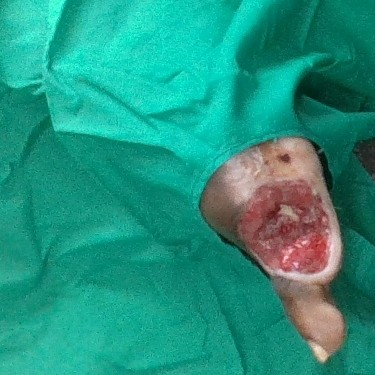
\includegraphics[width=.2\linewidth]{./Graphics/a.jpg}
	\end{subfigure}
	\begin{subfigure}
		\centering
		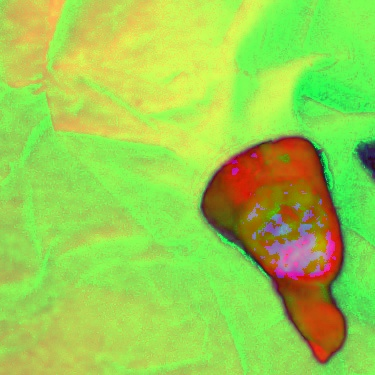
\includegraphics[width=.2\linewidth]{./Graphics/hsv.jpg}
	\end{subfigure}
	\begin{subfigure}
		\centering
		
\includegraphics[width=.2\linewidth]{./Graphics/tissue-mask.jpg}
	\end{subfigure}
	\begin{subfigure}
		\centering
		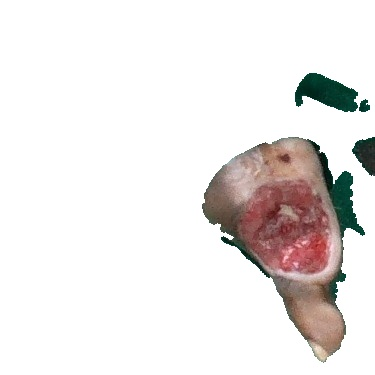
\includegraphics[width=.2\linewidth]{./Graphics/res.jpg}
	\end{subfigure}
	\caption{Proceso de segmentación del pañuelo para su eliminación automática: (1) se toma la imagen en RGB, (2) se convierte a HSV, (3) se seleccionan los píxeles por el umbral y (4) se aplica la máscara a la imagen en RGB.}
	\label{fig:tissue}
\end{figure}

Las imágenes RGB al ser obtenidas en un ambiente sin control de la iluminación y el enfoque pueden carecer del contraste suficiente o presentar ruido de emborronamiento (motion blur) producto del movimiento de la cámara. Por tales razones, se propone después de la etapa de captura aplicar el filtro de \textit{sharpening} y el mejoramiento de contraste usando el algoritmo CLAHE.



\section{Seguimiento de la zona de la UPD seleccionada de forma asistida}\label{segasis}

Las imágenes capturadas en el proceso anterior contienen demasiada información innecesaria para el algoritmo de segmentación propuesto por lo que se aumenta el umbral de error en la predicción. En las imágenes se captura la úlcera además de otros objetos presentes en el entorno pero que no son de interés para el algoritmo como son: herramientas de trabajo, el piso, utensilios y equipos médicos, entre otros. Por tal razón, se decidió adoptar un enfoque asistido para una pre-segmentación. 

El enfoque asistido consiste en que el especialista que captura la muestra centrará la atención del sistema en un área específica reduciendo el nivel de ruido e información excedente. El especialista que realiza la captura enmarcará la zona donde se encuentra la úlcera marcando mediante un rectángulo (o cuadrado) una zona de la imagen en cuyo centro se encuentra aproximadamente la UPD. Se utiliza el algoritmo de seguimiento de objetos en vídeo descrito en la Sección \ref{sec:csr} conocido como CSR-DCF. Con este enfoque se consigue una posición del cuadrado donde se encuentra la úlcera en cada cuadro o \textit{frame} de la muestra de vídeo. Estas subimágenes son las que se utilizan como entrada al algoritmo de segmentación.

\section{Segmentación}

En los procedimientos descritos en~\cite{wang2014smartphone, filko2018wound}, la segmentación de la UPD se ejecuta independiente y posterior a la reconstrucción 3D. Sin embargo, en este proyecto se trata desde otra perspectiva, que consiste en segmentar todas las imágenes RGB obtenidas en la captura para luego realizar la reconstrucción a partir de las máscaras que se obtienen. Al reconstruir utilizando las imágenes RGB luego de aplicar las máscara binaria, se logra una superficie de la escena donde solo tienen color las zonas de la úlcera, y el resto de los puntos aparecen en negro, luego estos puntos se eliminan para proceder a medir la malla.

Por tanto, el primer paso es ejecutar una segmentación de las imágenes RGB capturadas y recortadas por CSR-DCF. De cada una se obtiene una máscara, donde la zona de la lesión se exhibe en blanco y el resto en negro (Figura \ref{fig:dfuseg}). Estas imágenes junto con las originales RGB-D serán utilizadas en la reconstrucción para crear el modelo 3D sobre el cual se realizarán mediciones.

\begin{figure}[ht]
	\centering
	\begin{subfigure}
		\centering
		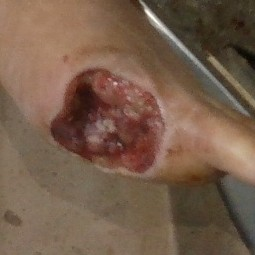
\includegraphics[width=.3\linewidth]{./Graphics/dfu.jpg}
	\end{subfigure}
	\begin{subfigure}
		\centering
		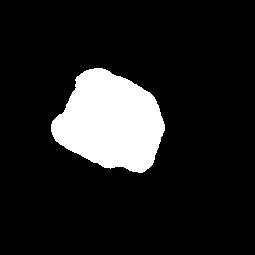
\includegraphics[width=.3\linewidth]{./Graphics/mask.jpg}
	\end{subfigure}
	\caption{Imágenes RGB de las úlceras y las máscaras de segmentación}
	\label{fig:dfuseg}
\end{figure}

La segmentación de las imágenes RGB puede ser lograda utilizando métodos tradicionales, como se explica en el capítulo \ref{chapter:state-of-the-art}. Sin embargo, estos están limitados por sus capacidades para la descripción de las características de las heridas. En la última década el Apredizaje Profundo ha adquirido popularidad en este ámbito. Toma ventaja de la poderosa habilidad de extracción de características de entrenadas Redes neuronales profundas (Deep Neural Networks, DNN) para el procesamiento de imágenes. Una desventaja es que requieren de grandes cantidades de datos durante el proceso de aprendizaje.

La redes neuronales UNet y LinkNet, descritas en la Sección \ref{sec:nn} del capítulo \ref{chapter:theoretical-framework}, son conocidas por sus buenos resultados en la tarea de segmentación de imágenes biomédicas y sin sacrificar el tiempo de procesamiento. En los artículos~\cite{chino2020segmenting, cui2019diabetic} se hace uso de las mismas para la segmentación de UPD y se muestran comparaciones con otros trabajos, respecto a los cuales se observan mejoras. Apoyándose en la generación de nuevas imágenes y en su arquitectura, brindan una alternativa favorable para el entrenamiento con pocos datos anotados. 

En el artículo~\cite{mahbod2021automatic} se propone emplear un conjunto de estas redes neuronales prediciendo en \textit{average ensemble}~\footnote{se dice de aquel predictor que su resultado depende del promedio de predictores anteriores.}. Se utilizan modelos pre-entrenados en los caminos de expansión en ambas arquitecturas. En el caso de la arquitectura UNet se utilizan los pesos del modelo EfficientNetB2~\cite{tan2019efficientnet} y en la arquitectura LinkNet se utilizan los pesos del modelo EfficientNetB1~\cite{tan2019efficientnet}, ambos modelos son pre-entrenados en el conjunto de datos Medetec~\cite{medetec}. En ese entrenamiento se utilizó la técnica de Aumento de Datos conocida como \textit{Data Augmentation} aplicando rotaciones y \textit{flips} en varios sentidos para obtener nuevas imágenes. En lugar de entrenar todas las redes sobre Medetec, se dividió el conjunto de datos en 5 subgrupos y se entrenó una red de cada arquitectura en cada uno de los subgrupos. Durante el proceso de predicción cada imagen pasa por cada uno de las 10 redes entrenadas y se obtienen 10 máscaras de segmentación semántica, luego se utiliza el promedio de las máscaras como predicción final. Luego de que se obtiene la máscara de segmentación se obtiene la imagen binaria de la misma y se le aplica un posprocesamiento, en el que se remueven los objetos bien pequeños y se rellenan los agujeros, aplicando la operación cerrado de morfología (Figura \ref{fig:pipeSeg}).

\begin{figure}[ht]
	\centering
	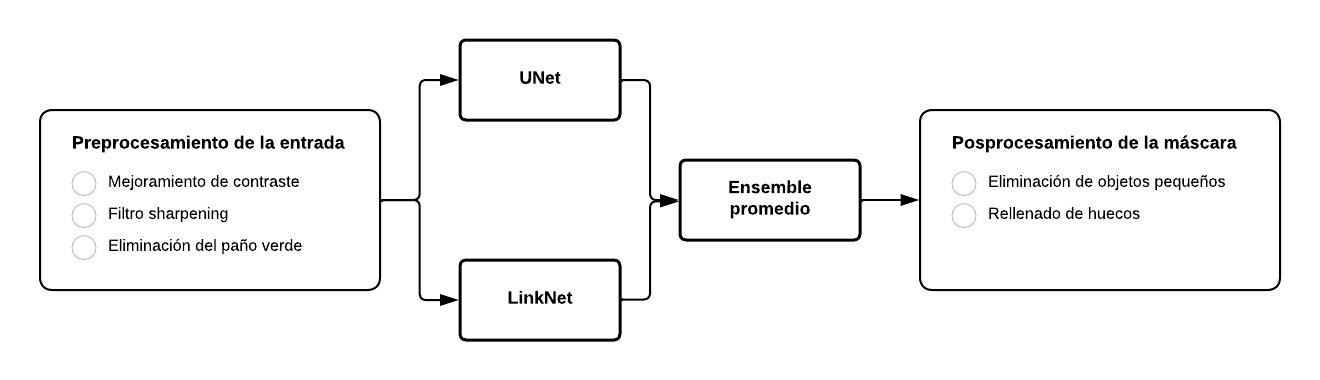
\includegraphics[width=12cm]{./Graphics/segmentation.png}
	\caption{Diagrama del algoritmo de segmentación propuesto}
	\label{fig:pipeSeg}
\end{figure}

\section{Reconstrucción 3D}

Para el proceso de reconstrucción 3D se plantea el uso del marco de trabajo (framework) \textit{Open3D}~\cite{zhou2018open3d}, una biblioteca de código abierto que expone un conjunto de estructuras de datos y algoritmos tanto en C++ como en Python. El \textit{back-end} está altamente optimizado y está configurado para la paralelización.

En \textit{Open3D} se proponen dos flujos de trabajo para la reconstrucción que se explican a continuación:

\begin{itemize}
	\item Basado en~\cite{dong2022ash} se formula un método en tiempo real u \textit{online}. Este realiza la reconstrucción volumétrica y un SLAM~\footnote{del inglés \textit{Simultaneous Localization and Mapping}} denso usando tensores y la interfaz de \textit{Hash Map} del propio \textit{Open3D}~\footnote{\textit{Open3D} permite paralelizar el \textit{hashing} tanto en la Unidad Gráfica de Procesamiento (GPU, por sus siglas en inglés) como en la Unidad Central de Procesamiento (CPU) usando llaves y valores organizados como tensores, donde se toma un lote de llave y/o valor como entrada}.
	\item Una reconstrucción a posterior u \textit{offline} completa de la escena a partir de una secuencia RGB-D. Esta está basada en~\cite{choi2015robust} y las ideas introducidas en~\cite{park2017colored} para una mejor reconstrucción.
\end{itemize}

A diferencia de los sistemas de reconstrucción en tiempo real, que no admiten alta complejidad, los \textit{offline} permiten el uso de algoritmos más complejos y demandantes desde el punto de vista computacional. Al no contar en esta propuesta con cámaras de una alta resolución (costo muy elevado) se pueden presentar errores de precisión.  Esto, sumado a la naturaleza estática de la escena, lleva a que un sistema de reconstrucción 3D \textit{offline} brinde mejoras en la calidad de los modelos 3D finales. 

En la Sección \ref{section:rec3dmet} se describe el funcionamiento de este sistema. La entrada consiste en la matriz intrínseca junto con la secuencia de imágenes RGB-D a reconstruir. La matriz se construye con los parámetros intrínsecos de la cámara, calculados mediante el proceso de auto-calibración descrito en la sección \ref{section:calibration}. Para alinear las imágenes de color con las de profundidad se realiza una transformación geométrica por píxel en función de los datos de profundidad proporcionados. 

Con estos datos de entrada el sistema estima la posición de cada imagen RGB-D en el espacio global; posteriormente, se integran en un solo volumen TSDF que brinda como resultado un modelo 3D que describe la escena, representado a través de una malla poligonal a colores.

\begin{figure}[ht]
	\centering
	\begin{subfigure}
		\centering
		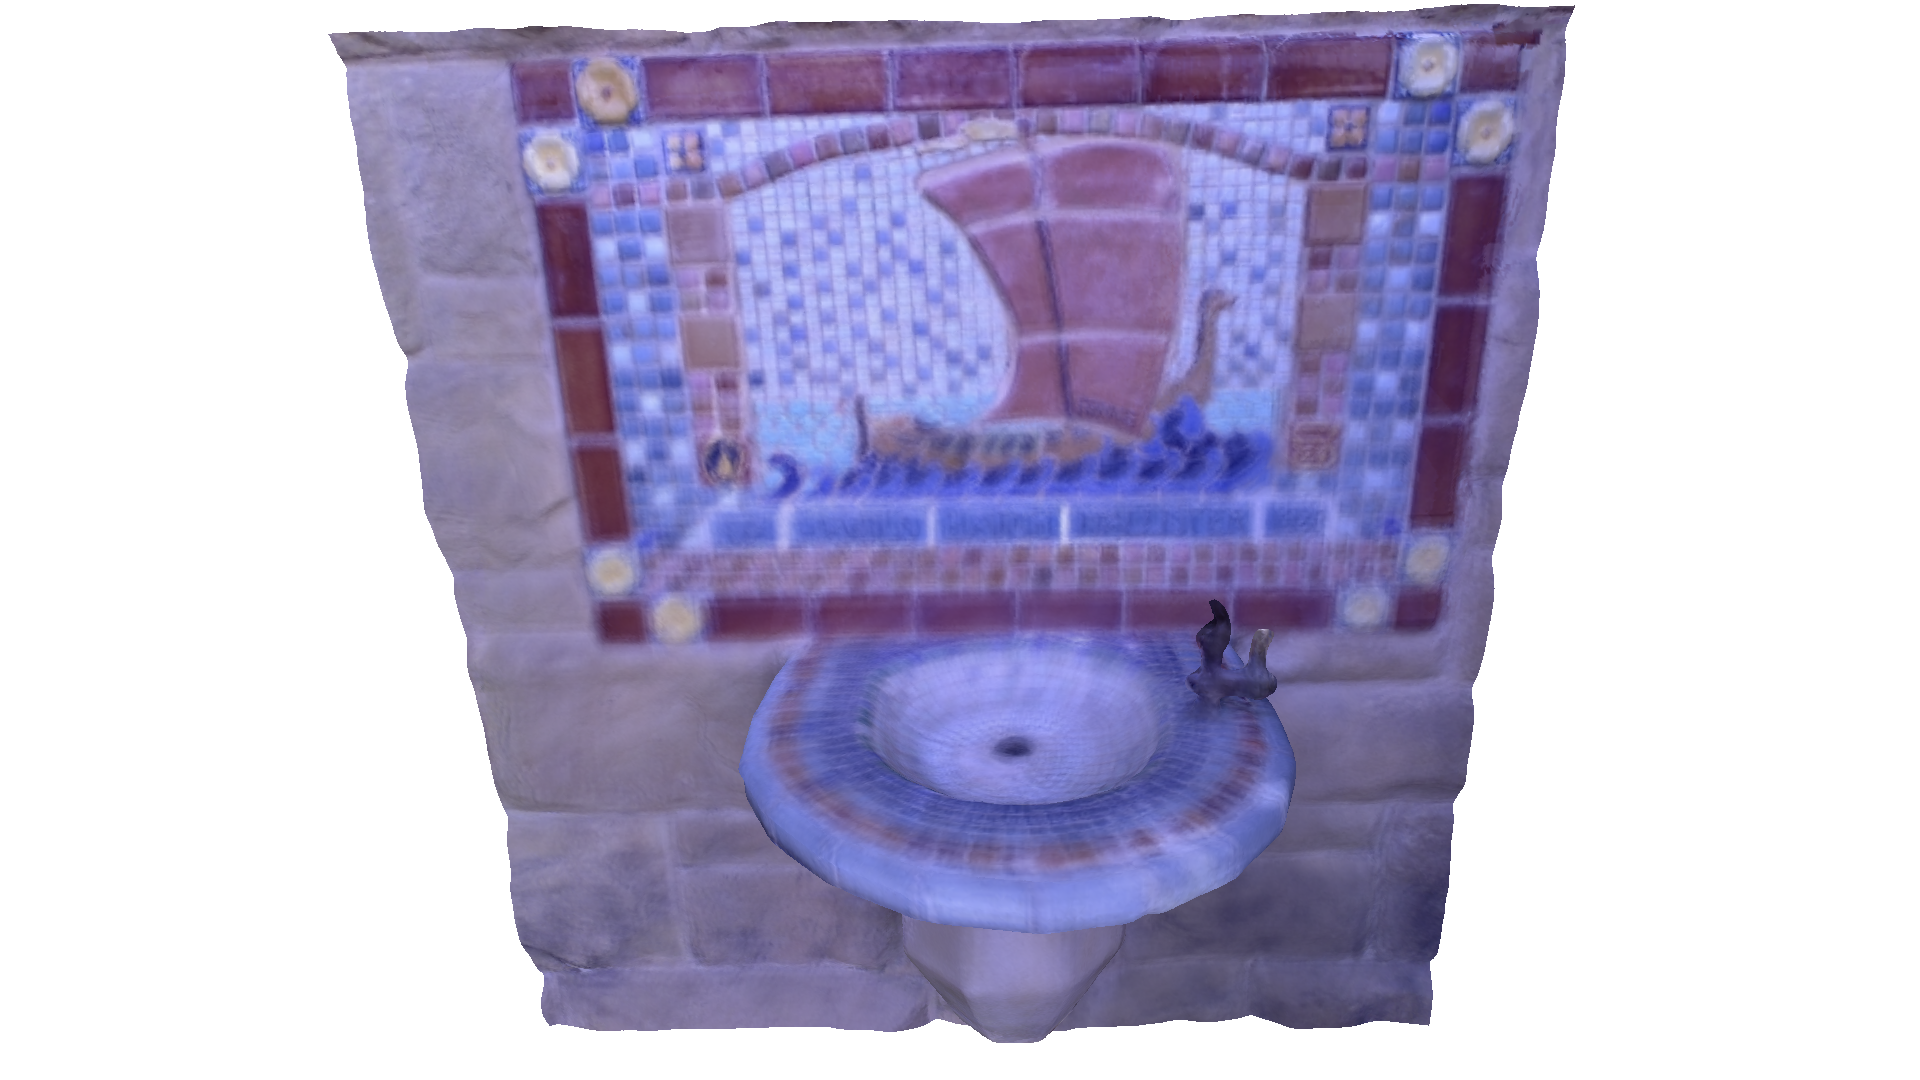
\includegraphics[width=.4\linewidth]{./Graphics/co1.png}
	\end{subfigure}
	\begin{subfigure}
		\centering
		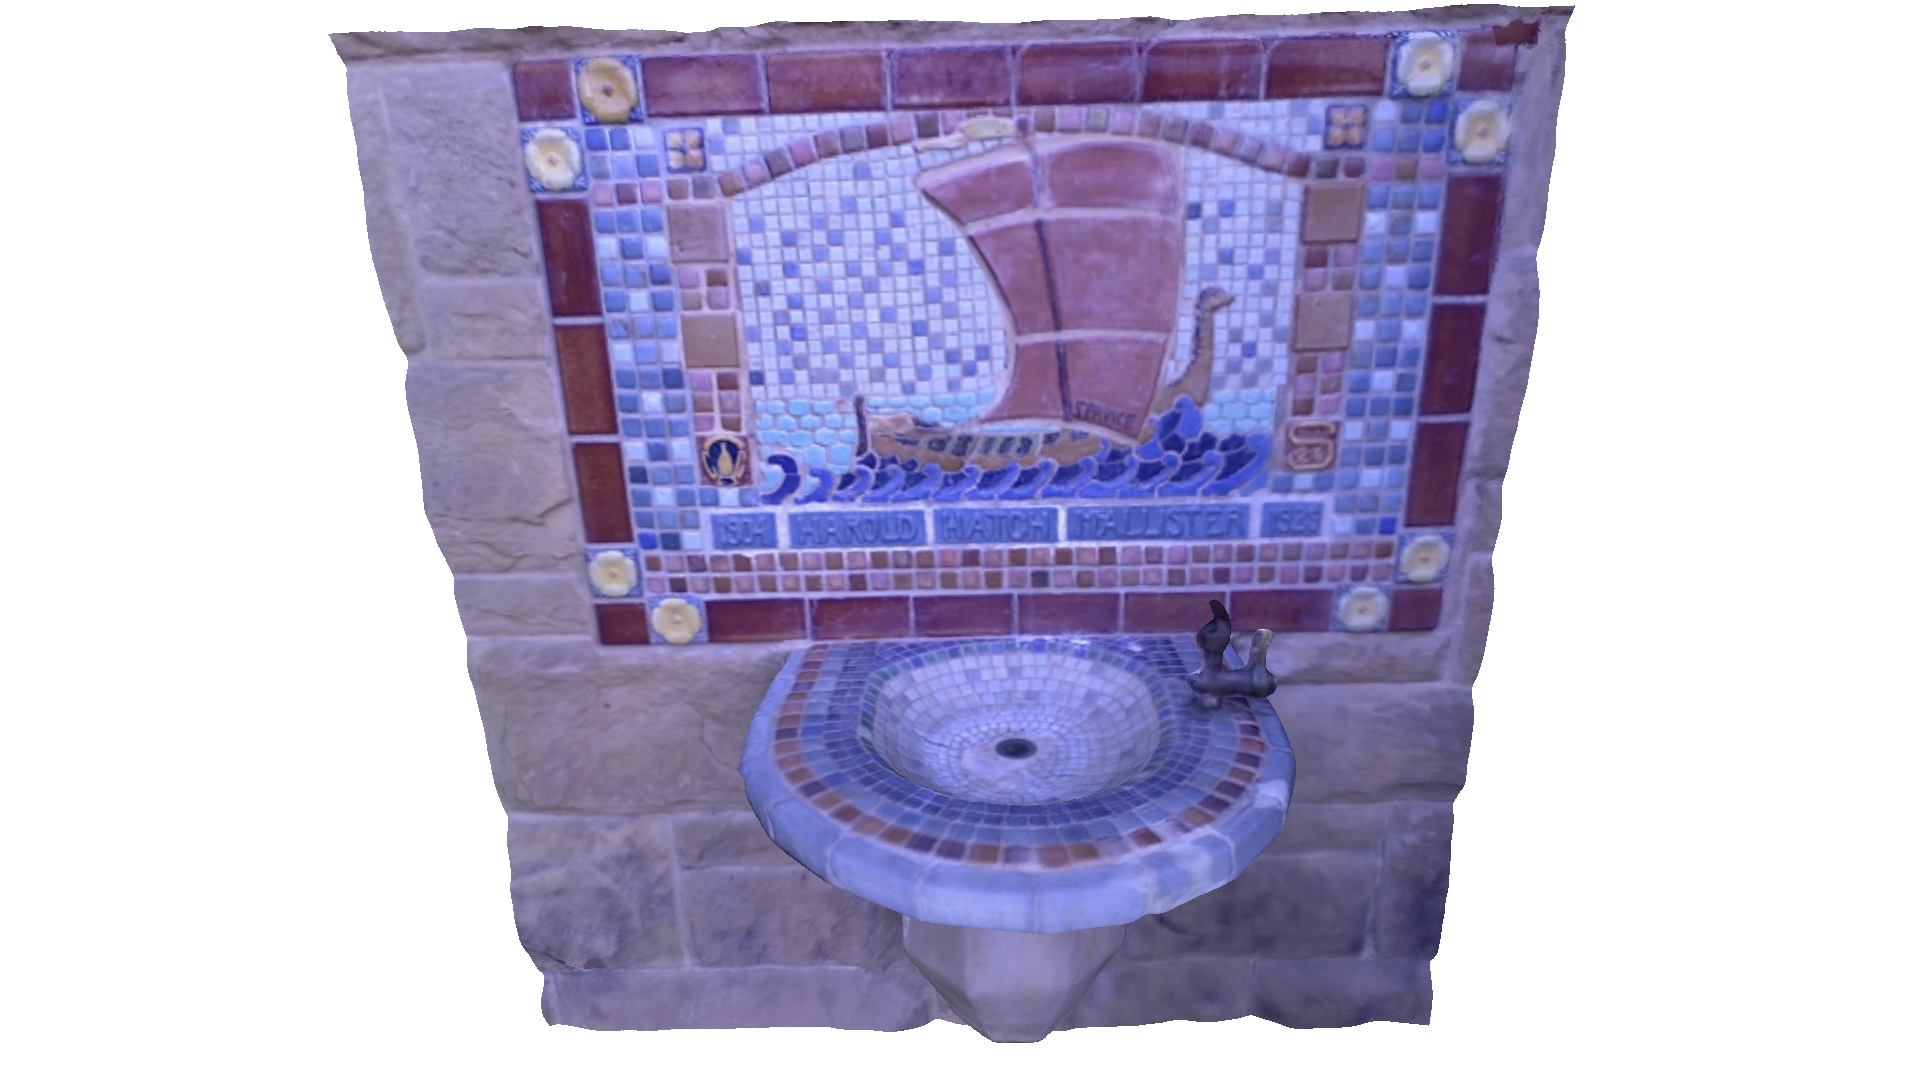
\includegraphics[width=.4\linewidth]{./Graphics/co2.png}
	\end{subfigure}
	\caption{Resultado del método de optimización de mapas de color propuesto en~\cite{zhou2014color}.}
	\label{fig:optColor3d}
\end{figure}

Dado que los marcos de color y profundidad no están perfectamente alineados si se hacen corresponder los colores a la geometría reconstruida la correspondencia de texturas puede resultar en un mapa de color borroso (Figura \ref{fig:optColor3d}). La biblioteca \textit{Open3D} proporciona para este caso el método de optimización de mapas de color propuesto por~\cite{zhou2014color}. Pero se necesita un segundo modelo que defina la segmentación 3D. Para lograrlo se modifica el último paso de la reconstrucción, la integración de la escena. Esta vez se sustituyen las imágenes RGB por las máscaras resultantes de la segmentación 2D aplicadas a las imágenes de color y se aprovecha la estimación de la posición global obtenidas de los fragmentos registrados con las imágenes de color sin segmentar. De esta forma se adquiere una malla que solo presenta colores en la región segmentada, para luego eliminar de esta todo vértice que tenga un color negro puro y las aristas que unen a los mismos.

\section{Mediciones}

La propuesta para las mediciones utiliza los algoritmos presentados en la Sección \ref{section:measure}. Se recibe un archivo \texttt{.ply} con el modelo resultante de la reconstrucción 3D. De este modelo se extrae la nube de puntos y la malla poligonal del modelo para realizar la medición. La escala de las coordenadas de los puntos se fija en milímetros (mm) a través del parámetro \texttt{DEPTH\_UNITS} en la cámara. Este parámetro representa el número de metros por unidad de profundidad. Luego, las mediciones en el sistema se expresan en milímetros.

Para el perímetro se trabaja sobre la nube de puntos del modelo. Se construye una nube de puntos en 2D, anulando la componente de profundidad $z$. Esto con el fin de calcular la envoltura convexa en esta nueva nube de puntos, y obtener los puntos que están en la envoltura convexa, o sea, los puntos frontera. Luego, se calcula la distancia entre estos puntos. Al eliminar la componente $z$ de la nube de puntos no se afecta la precisión de la medición pues se mantiene la noción de distancia en el plano $XY$ obtenida de la reconstrucción, la cual es suficiente a la hora de estimar el perímetro.  

Para el área se trabaja con la malla poligonal del modelo, calculando el área total como la sumatoria del área de los triángulos de la malla, utilizando la fórmula de Herón. Luego, se divide el resultado entre \texttt{DEPTH\_UNITS}$^2$ para obtener el área.

Para el volumen se trabaja con la nube de puntos, se calcula la envoltura convexa de la nube de puntos y se realiza la interpolación de la tapa, y luego se realiza la triangulación de Delaunay entre la tapa y la úlcera. Posteriormente se procede a calcular el volumen total como la sumatoria del volumen de las pirámides resultantes. Luego, se divide el resultado entre \texttt{DEPTH\_UNITS}$^3$ para obtener el volumen. 


\section{Flujo de trabajo del programa}

En las secciones anteriores se han descrito los flujos de trabajo de las distintas etapas del sistema. El programa propuesto no es más que una aplicación de consola, donde se reciben los datos relativos al paciente, tales como: nombre, edad, sexo, tipo de diabetes y localización de la úlcera. Luego se procede a capturar la muestra utilizando la cámara de profundidad, asistida por el algoritmo de seguimiento o rastreo de objetos en secuencias de vídeo. Posteriormente, se obtienen las imágenes RGB de la escena, las imágenes comprendidas dentro de \textquotedblleft la caja\textquotedblright\ de seguimiento y las imágenes de profundidad de la escena. Las imágenes del interior de la caja se proveen como entrada al algoritmo de segmentación y se obtienen las máscaras correspondientes. Estas máscaras de segmentación se amplían hasta la resolución de las imágenes de la escena, se toma la región segmentada y se introduce al algoritmo de reconstrucción 3D junto a las imágenes de profundidad. La reconstrucción retorna un modelo 3D de la escena, se elimina toda la información no relacionada con la región segmentada en el modelo. Sobre este modelo segmentado se realizan las mediciones correspondientes al perímetro, el área y el volumen. Como finalización del flujo se exporta un archivo \verb|.pdf| con la información del paciente y las mediciones. 

\begin{figure}[h]
	\centering
	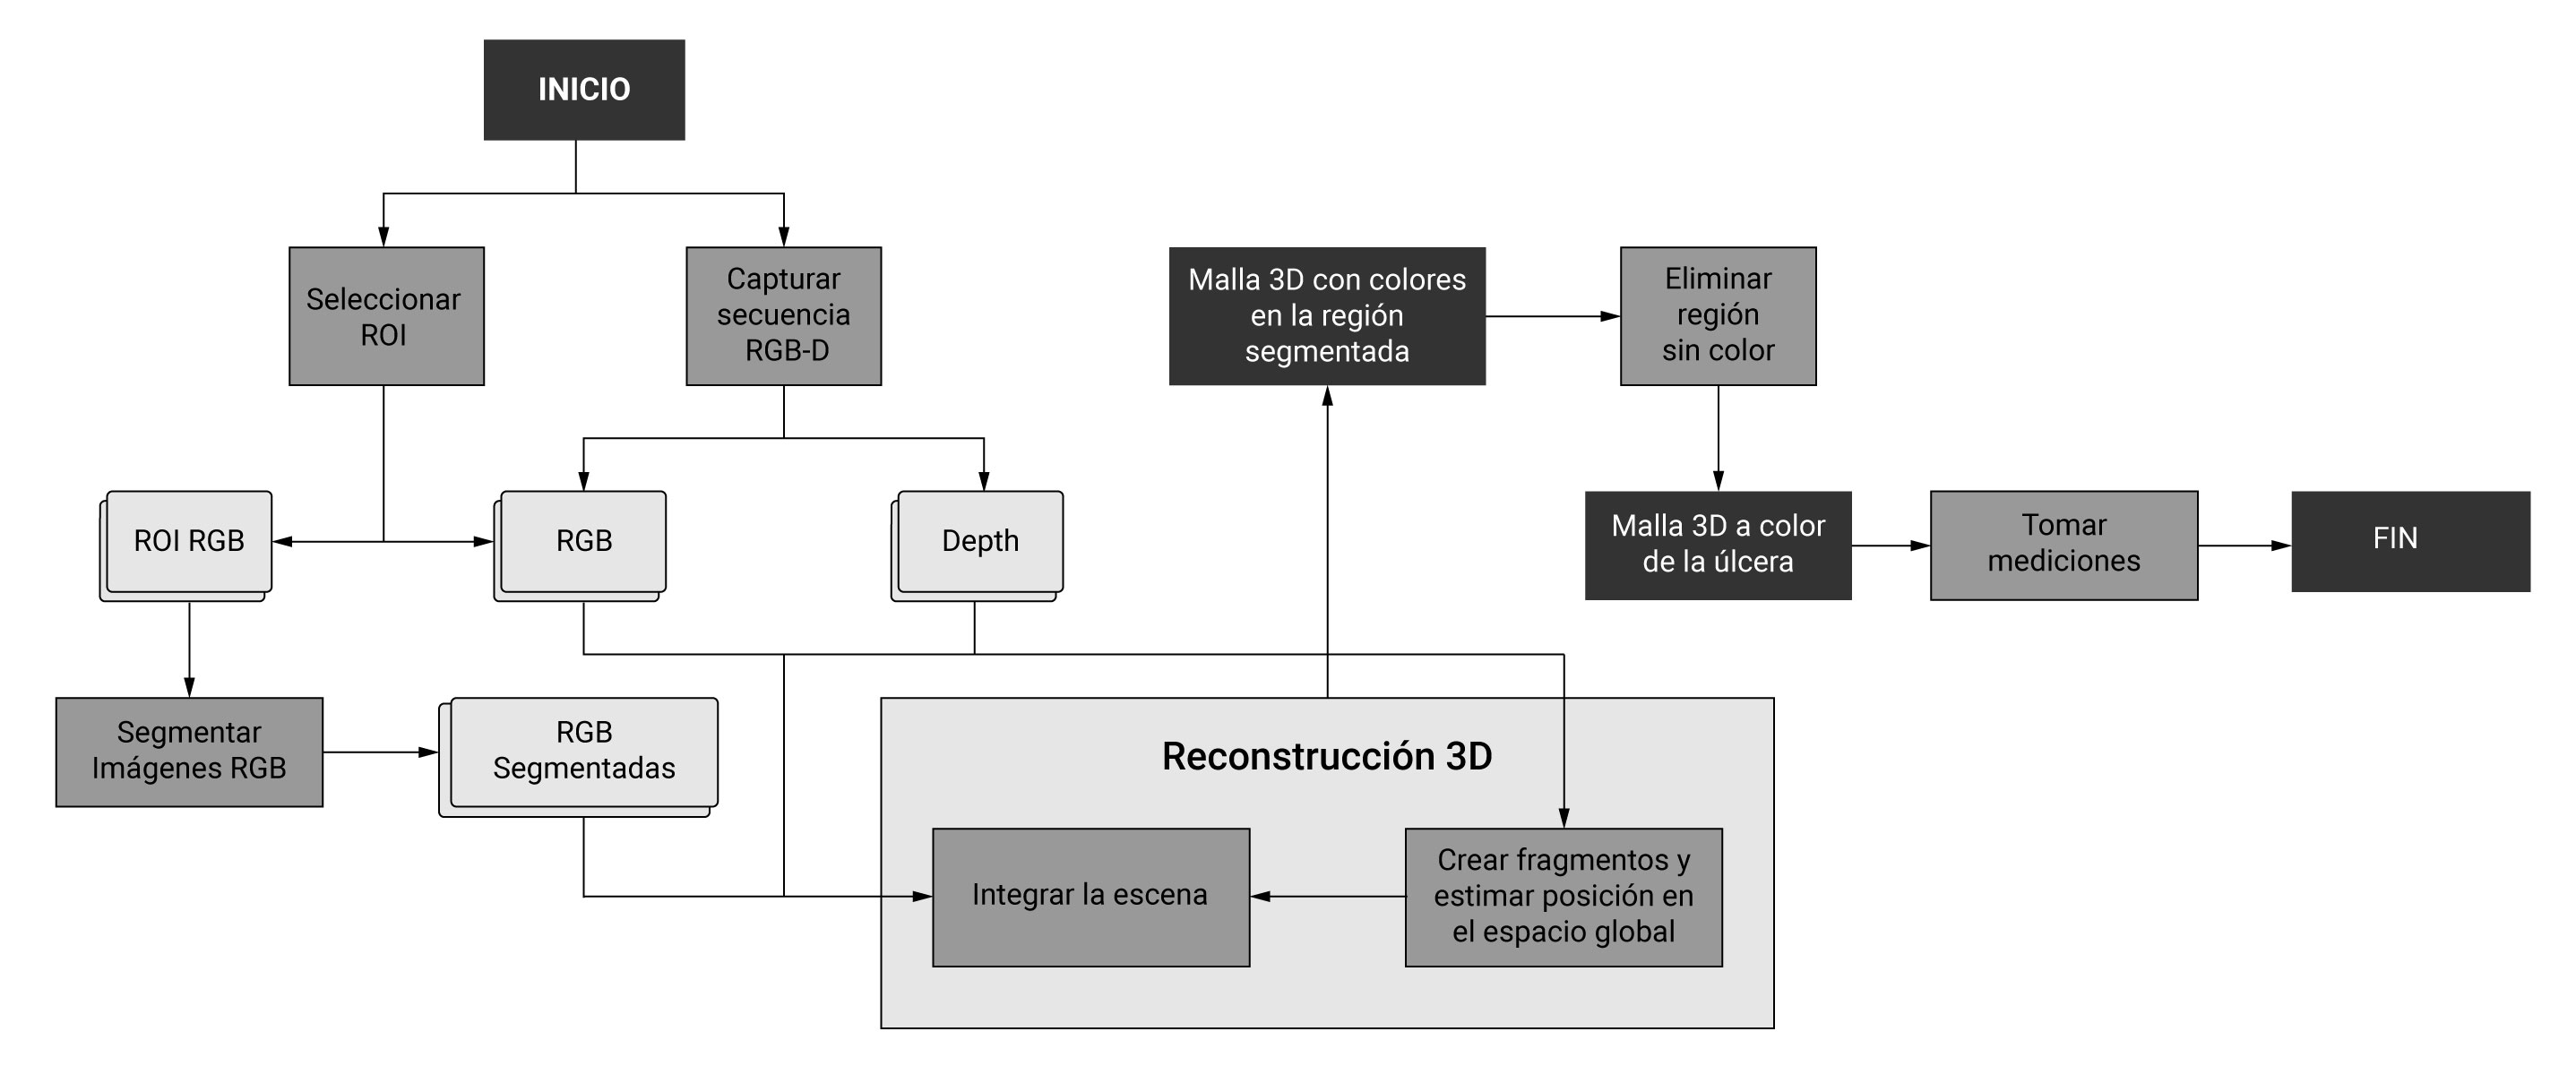
\includegraphics[width=15cm]{./Graphics/flow.jpg}
	\caption{Diagrama de flujo de la aplicación propuesta}
	\label{fig:flowCLI}
\end{figure}